\documentclass[10pt,a4paper]{article}
\usepackage[margin=2.2cm]{geometry}
\usepackage{amsmath,amssymb}
\usepackage{booktabs,tabularx,array,multirow}
\usepackage{xcolor}
\usepackage{tikz}
\usepackage{fancyhdr}
\usepackage{titlesec}
\usepackage{enumitem}
\usepackage[hidelinks]{hyperref}
\usepackage{tcolorbox}

\definecolor{accent}{HTML}{1F4E79}
\definecolor{keybg}{HTML}{EEF3F6}
\definecolor{cmag}{HTML}{1F6F8B}
\definecolor{cfis}{HTML}{6A8F3A}
\definecolor{cgrad}{HTML}{C0612B}
\definecolor{crand}{HTML}{8A939C}

\newcommand{\best}[1]{\textcolor{cmag}{\textbf{#1}}}

\titleformat{\section}{\large\bfseries\color{accent}}{\thesection}{0.6em}{}
\titleformat{\subsection}{\normalsize\bfseries}{\thesubsection}{0.5em}{}
\setlist{itemsep=2pt,topsep=3pt}

\pagestyle{fancy}
\fancyhf{}
\fancyhead[L]{\small Reliable and Secure ReRAM Crossbar Accelerators}
\fancyhead[R]{\small CS5290 -- Phase 1 Results}
\fancyfoot[C]{\small\thepage}

\begin{document}

\begin{center}
{\small CS5290 Memory-Centric Computer Architecture $\cdot$ Results Report (24 October 2026)}\\[6pt]
{\LARGE\bfseries Protecting the Right Weights on a Noisy ReRAM Chip}\\[6pt]
{\large Phase 1 results for BERT-Base and DistilBERT on a hybrid SLC/MLC crossbar (plan tasks 1--7)}
\end{center}

\begin{tcolorbox}[colback=keybg,colframe=accent,boxrule=0.5pt,arc=1pt,left=6pt,right=6pt,top=4pt,bottom=4pt,
  title={Main findings},fonttitle=\bfseries\small,coltitle=white]
\begin{enumerate}[leftmargin=*]
\item Storing a transformer only in dense two-bit cells (MLC) does not work. At realistic programming
noise, BERT-Base drops from 90\% to close to coin-flip accuracy.
\item Keeping a small share of the weight components in reliable one-bit cells (SLC) recovers almost all of
this loss, as HyFlexPIM proposes. It only works if the right components are chosen.
\item The simplest choice, keeping the components with the \textbf{largest singular values}, works best. It
beats the gradient-based choice used by HyFlexPIM at every SLC share, every noise level and on both
models.
\item With this choice, 5--10\% of components in SLC is enough at 5\% noise, and about 30\% at 7.5\% noise.
This needs roughly 60--70\% of the memory cells of an all-SLC chip, with no loss of accuracy.
\end{enumerate}
\end{tcolorbox}

\section{The Problem}
A ReRAM crossbar runs a neural network inside the memory. Each weight is stored as the conductance of
resistive cells, and a matrix--vector product happens in one step as currents add up along the wires.
This avoids most of the data movement that dominates the energy of conventional hardware. The difficulty
is that a cell cannot be programmed to an exact conductance, so every stored weight carries some random
error.

A cell can store one bit (SLC) or several bits (MLC). SLC has only two well-separated levels and
tolerates noise well. MLC packs more levels into the same range, so it is denser but the same noise does
more damage. In our set-up an 8-bit weight needs 7 SLC cells or 4 MLC cells for each sign.

HyFlexPIM (ISCA 2025) proposes a middle path. Each weight matrix is split with singular value
decomposition (SVD) into components, the most important $\sim$20\% are stored in SLC and the rest in MLC.
HyFlexPIM decides importance from the gradient of the loss with respect to each singular value.

We asked two questions: does this hybrid scheme hold up in a bit-accurate simulation of the hardware,
and is the gradient the right way to decide which components to protect?

\section{How We Tested It}
We used two pretrained sentiment classifiers, \textbf{BERT-Base} (72 weight matrices placed on the
crossbar) and \textbf{DistilBERT} (36), and scored them on all 872 validation sentences of the SST-2
movie-review task. All runs used Kaggle GPUs.

\begin{description}[leftmargin=1.2em,labelindent=0pt]
\item[SVD step.] Each matrix is factorised (384 components for a $768\times768$ layer), and the model is
fine-tuned for 8 epochs to recover accuracy.
\item[Simulator.] 8-bit weights are stored on a pair of crossbars (positive and negative parts) and split
across cells. Inputs are 8-bit. The analog-to-digital converter (ADC) is treated as ideal for now.
\item[Noise $\sigma$.] Random programming error added to every cell, given as a percentage of the maximum
conductance. Values of 2--10\% are typical in the literature.
\item[Simulated chip.] One random draw of all cell errors. Results are averaged over 5 chips (task 6) or
20 chips (task 7), and we also look at the worst chip.
\end{description}

\noindent We compared four ways of choosing which components go to SLC, plus the two extremes (everything
in SLC and everything in MLC):
\begin{itemize}
\item \textbf{Gradient:} the HyFlexPIM score, the loss gradient summed over 2{,}048 training sentences.
\item \textbf{Magnitude:} simply the size of the singular value.
\item \textbf{Fisher:} the gradient squared for each sentence before summing, so positive and negative
contributions cannot cancel. We added it to explain the gradient result.
\item \textbf{Random:} a control showing what happens with no ranking at all.
\end{itemize}
The SVD and fine-tuning are done once. Changing the SLC share or the ranking only changes which cells
each component is stored in, never the weights themselves, so every comparison uses the same model.

\section{Starting Point: the Cost of SVD}

\begin{table}[h]
\centering\small
\begin{tabular}{@{}lcccc@{}}
\toprule
Model & Original FP32 & Original INT8 & SVD, before fine-tune & SVD, after fine-tune \\
\midrule
BERT-Base  & 92.43 & 91.86 & 89.33 & 90.14 \\
DistilBERT & 91.06 & 90.37 & 89.68 & 89.11 \\
\bottomrule
\end{tabular}
\caption{SST-2 accuracy (\%) with no hardware error. INT8 is the original model with the same layers
quantised to 8 bits.}
\end{table}

Quantising to 8 bits costs only about 0.6 points, so 8-bit storage is not the issue. The SVD step costs
more: 2.3 points for BERT-Base and 2.0 for DistilBERT, even after fine-tuning. Fine-tuning helped
BERT-Base but slightly hurt DistilBERT, which suggests over-fitting. This gap is a fixed cost of the
HyFlexPIM approach in our implementation, paid before any hardware error.

With no noise, the simulated chip matched the SVD model to within 0.5 points for every placement, which
confirmed that the simulator adds no hidden error of its own.

\section{Programming Noise with 20\% in SLC}
We first fixed the SLC share at HyFlexPIM's 20\% and increased the noise.

\begin{table}[h]
\centering\small
\begin{tabular}{@{}lcccccc@{}}
\toprule
Placement & $\sigma=0$ & 2\% & 3\% & 5\% & 7.5\% & 10\% \\
\midrule
All SLC & 89.9 & 89.3 & 89.1 & 87.8 & 85.9 & 79.7 \\
All MLC & 90.0 & 87.3 & 83.9 & 66.3 & 52.2 & 51.3 \\
\midrule
Gradient, 20\% SLC  & 90.3 & 89.7 & 89.5 & 85.8 & 72.1 & 60.3 \\
Magnitude, 20\% SLC & 89.7 & \best{89.9} & \best{90.0} & \best{88.6} & 83.5 & 72.0 \\
Random, 20\% SLC    & 90.0 & 89.9 & 87.7 & 78.8 & 58.8 & 49.1 \\
\bottomrule
\end{tabular}
\caption{BERT-Base, mean accuracy (\%) over 5 chips. DistilBERT behaves the same way but is somewhat more
tolerant: all-MLC holds 74.5\% at $\sigma=5\%$, against 66.3\% for BERT-Base.}
\end{table}

Three things stand out. All-MLC collapses once noise reaches 5\%. Protecting 20\% of the components fixes
most of the damage, but random selection fixes little, so \emph{which} components are protected matters
more than how many. And magnitude selection beat the gradient method that HyFlexPIM recommends, by
2.8 points at 5\% noise and 11.4 points at 7.5\%. Because this contradicted the paper, we tested it more
carefully in the next experiment.

\section{How Much SLC Is Needed?}
We then varied the SLC share from 5\% to 50\% at three noise levels, with 20 chips per point.

\begin{figure}[h]
\centering
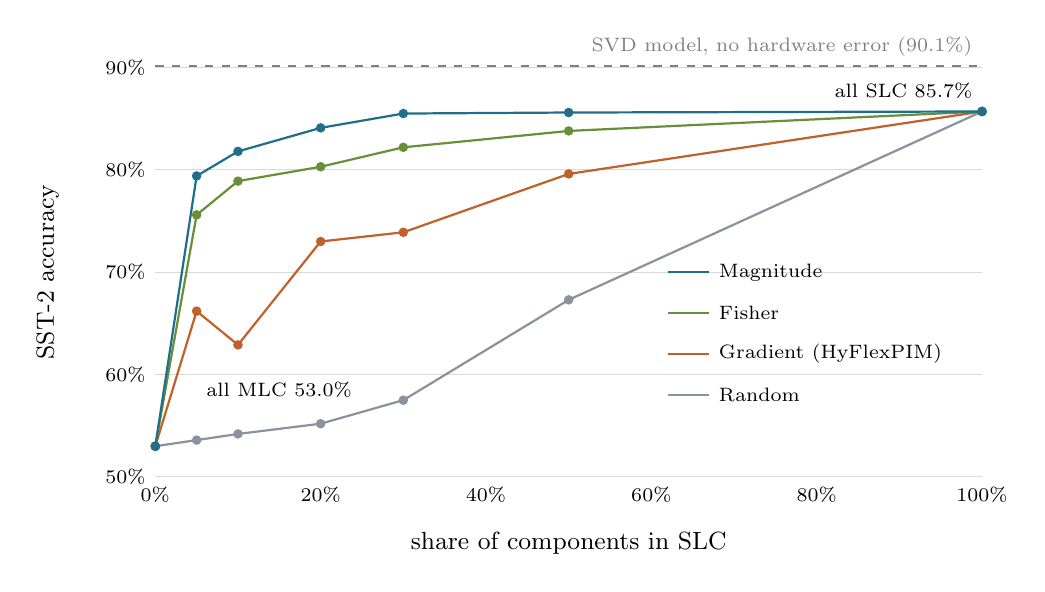
\begin{tikzpicture}[x=0.105cm,y=0.13cm]
  % axes: x = SLC share 0..100 %, y = accuracy 50..90 % (shifted by 50)
  \foreach \v in {50,60,70,80,90} {
    \draw[gray!30] (0,\v-50) -- (100,\v-50);
    \node[left,font=\scriptsize] at (0,\v-50) {\v\%};
  }
  \foreach \v in {0,20,40,60,80,100}
    \node[below,font=\scriptsize] at (\v,0) {\v\%};
  \node[font=\small] at (50,-6.5) {share of components in SLC};
  \node[rotate=90,font=\small] at (-13,20) {SST-2 accuracy};
  \draw[gray,dashed] (0,40.14) -- (100,40.14);
  \node[above left,font=\scriptsize,gray] at (100,40.14) {SVD model, no hardware error (90.1\%)};
  % series: all-MLC 53.0 at 0, all-SLC 85.7 at 100
  \draw[crand,thick] plot[mark=*,mark size=1.3pt] coordinates
    {(0,3.0) (5,3.6) (10,4.2) (20,5.2) (30,7.5) (50,17.3) (100,35.7)};
  \draw[cgrad,thick] plot[mark=*,mark size=1.3pt] coordinates
    {(0,3.0) (5,16.2) (10,12.9) (20,23.0) (30,23.9) (50,29.6) (100,35.7)};
  \draw[cfis,thick] plot[mark=*,mark size=1.3pt] coordinates
    {(0,3.0) (5,25.6) (10,28.9) (20,30.3) (30,32.2) (50,33.8) (100,35.7)};
  \draw[cmag,thick] plot[mark=*,mark size=1.3pt] coordinates
    {(0,3.0) (5,29.4) (10,31.8) (20,34.1) (30,35.5) (50,35.6) (100,35.7)};
  \node[right,font=\scriptsize] at (5,8.5) {all MLC 53.0\%};
  \node[above left,font=\scriptsize] at (100,36.0) {all SLC 85.7\%};
  % legend
  \begin{scope}[shift={(62,8)},font=\scriptsize]
    \draw[cmag,thick] (0,12) -- (5,12); \node[right] at (5,12) {Magnitude};
    \draw[cfis,thick] (0,8) -- (5,8);   \node[right] at (5,8) {Fisher};
    \draw[cgrad,thick] (0,4) -- (5,4);  \node[right] at (5,4) {Gradient (HyFlexPIM)};
    \draw[crand,thick] (0,0) -- (5,0);  \node[right] at (5,0) {Random};
  \end{scope}
\end{tikzpicture}
\caption{BERT-Base at $\sigma=7.5\%$, mean of 20 chips. The 0\% and 100\% points are all-MLC and all-SLC,
shared by every ranking.}
\end{figure}

\begin{table}[h]
\centering\small
\begin{tabular}{@{}llcccccc@{}}
\toprule
Noise & Ranking & 5\% & 10\% & 20\% & 30\% & 50\% & All SLC \\
\midrule
\multirow{4}{*}{$\sigma=5\%$}
 & Magnitude & \best{88.0} & \best{88.6} & \best{88.7} & \best{88.9} & \best{88.9} & \multirow{4}{*}{88.0} \\
 & Fisher    & 87.3 & 87.9 & 88.1 & 88.3 & 88.4 & \\
 & Gradient  & 83.0 & 82.0 & 86.5 & 86.1 & 88.1 & \\
 & Random    & 72.5 & 73.6 & 76.2 & 77.8 & 83.4 & \\
\midrule
\multirow{4}{*}{$\sigma=7.5\%$}
 & Magnitude & \best{79.4} & \best{81.8} & \best{84.1} & \best{85.5} & \best{85.6} & \multirow{4}{*}{85.7} \\
 & Fisher    & 75.6 & 78.9 & 80.3 & 82.2 & 83.8 & \\
 & Gradient  & 66.2 & 62.9 & 73.0 & 73.9 & 79.6 & \\
 & Random    & 53.6 & 54.2 & 55.2 & 57.5 & 67.3 & \\
\bottomrule
\end{tabular}
\caption{BERT-Base, mean accuracy (\%) over 20 chips, by share of components in SLC. All-MLC scores 66.8\%
($\sigma=5\%$) and 53.0\% ($\sigma=7.5\%$).}
\end{table}

\subsection{Magnitude is consistently the best ranking}
The order magnitude $>$ Fisher $>$ gradient $>$ random held at all 15 combinations of SLC share and
noise level, on both models. The gap is widest where it matters most, on the worst chip. At
$\sigma=7.5\%$ with 20\% in SLC, the worst of 20 BERT-Base chips scored 76.0\% with magnitude, 72.1\% with
Fisher and 49.8\% with gradient, which is no better than random. The gradient ranking is also unstable:
for BERT-Base, raising the SLC share from 5\% to 10\% made results \emph{worse} at both 5\% and 7.5\%
noise, which should not happen if the ranking reflected true importance.

\subsection{Why the gradient method falls short}
The fine-tuned model sits close to a minimum of the loss. There, the gradient for a given component is
positive on some sentences and negative on others, and summing them lets these cancel. An important
component can then receive a small score. The Fisher score avoids this by squaring before summing. Fisher
closed most of the gap to magnitude (at $\sigma=7.5\%$ and 20\% SLC: gradient 73.0, Fisher 80.3,
magnitude 84.1), so sign cancellation explains a large part of the problem.

It does not explain all of it, since magnitude still wins. Our working explanation is that gradient and
Fisher scores measure how sensitive the loss is to a \emph{small} change in a component, while hardware
noise is not small. Programming error is a fixed fraction of the conductance range, so the absolute error
a component carries grows with its size, and the components with the largest singular values may be the
ones that suffer most when left in MLC. This hypothesis has not been tested yet.

\subsection{The SLC budget depends on the noise level}
With magnitude ranking, the SLC share needed to come within half a point of an all-SLC chip was:
\begin{itemize}
\item $\sigma=3\%$: 5\% is already enough. Every ranking except random is within about one point of
all-SLC here.
\item $\sigma=5\%$: 5--10\%. Above 10\% the hybrid chip scores 88.6--88.9\% against 88.0\% for all-SLC.
This small advantage is within the chip-to-chip spread, so we treat it as a tie.
\item $\sigma=7.5\%$: about 30\% (85.5\% against 85.7\%). Gradient is still 6 points short at 50\%.
\end{itemize}
DistilBERT followed the same pattern. At $\sigma=7.5\%$ it needed 30--50\% SLC with magnitude
(86.6--86.9\% against 87.4\%), while gradient reached only 84.4\% at 50\%.

\subsection{What this saves in hardware}
Counting only the cells that store weights, a chip with a share $f$ in SLC needs $7f + 4(1-f)$ cells per
weight, against 7 for an all-SLC chip. At 10\% SLC this is 61\% of the all-SLC cell count, at 30\% it is
70\%, and an all-MLC chip would be 57\%. At moderate noise, a magnitude-ranked hybrid chip therefore comes
close to MLC density while keeping SLC accuracy. A full area and energy estimate, including ADCs and other
circuitry, is planned for task 15.

\section{Conclusions}
\begin{itemize}
\item Storing a transformer purely in two-bit cells is not viable at realistic noise, so a hybrid SLC/MLC
layout is necessary.
\item HyFlexPIM's hybrid idea works in our bit-accurate simulation, but its gradient-based ranking is not
the best way to choose protected components. Ranking by singular value is simpler, needs no training
data, and gives higher and more consistent accuracy across chips.
\item The SLC share should be chosen for the expected noise: around 10\% at moderate noise and around 30\%
at high noise.
\item From task 8 onward we use magnitude ranking as the default, and keep gradient ranking as the
HyFlexPIM baseline for comparison.
\end{itemize}

\section{Limitations and Open Questions}
\begin{itemize}
\item The simulator so far models only programming noise. The ADC is ideal, inputs are applied all at
once rather than bit by bit, and read noise, wire resistance (IR drop) and faulty cells are not yet
included. These could change how the methods rank.
\item The 2-point SVD loss still needs to be compared with the figure reported by HyFlexPIM, and
DistilBERT's fine-tuning needs early stopping.
\item The explanation for why magnitude beats Fisher is untested.
\item All results are on a single task (SST-2). MRPC and the CNN models follow in Phase 2.
\end{itemize}

\section{Progress and Next Steps}

\begin{table}[h]
\centering\small
\begin{tabularx}{\linewidth}{@{}lXl@{}}
\toprule
Task & Description & Status \\
\midrule
1--2  & FP32 and INT8 baselines & Done \\
3     & HyFlexPIM SVD pipeline & Done \\
4--5  & Crossbar simulator and end-to-end check & Done \\
6     & Placement vs.\ programming noise & Done \\
7     & Accuracy vs.\ SLC share, with Fisher ranking & Done \\
8     & Stuck-at faults (0--5\% of cells) & Running \\
9     & Realistic ADC, bit-serial inputs, read noise, clustered faults, IR drop & Next \\
10--15 & Noise-aware training, fault-aware mapping, contributions C1--C4, hardware cost & Planned \\
\bottomrule
\end{tabularx}
\end{table}

Task 8 tests whether these findings survive a different kind of error. A stuck cell always reads fully
on or fully off. SLC uses more cells per weight and so has more cells that can fail, while a stuck MLC
cell causes a larger error. It is not yet clear whether SLC protection, or magnitude ranking, still helps
when cells fail outright.

\vspace{6pt}
\noindent{\footnotesize\color{gray} Models: textattack/bert-base-uncased-SST-2 and
distilbert-base-uncased-finetuned-sst-2-english. Simulator: 8-bit weights, on/off ratio 100, differential
cell pairs, 128-row tiles. Ranking scores computed on 2{,}048 SST-2 training sentences.}

\end{document}
